\documentclass[smaller]{beamer}

\usepackage{eecs}

\usepackage{etex}
\usepackage[all]{xy}


%% ODER: format ==         = "\mathrel{==}"
%% ODER: format /=         = "\neq "
%
%
\makeatletter
\@ifundefined{lhs2tex.lhs2tex.sty.read}%
  {\@namedef{lhs2tex.lhs2tex.sty.read}{}%
   \newcommand\SkipToFmtEnd{}%
   \newcommand\EndFmtInput{}%
   \long\def\SkipToFmtEnd#1\EndFmtInput{}%
  }\SkipToFmtEnd

\newcommand\ReadOnlyOnce[1]{\@ifundefined{#1}{\@namedef{#1}{}}\SkipToFmtEnd}
\usepackage{amstext}
\usepackage{amssymb}
\usepackage{stmaryrd}
\DeclareFontFamily{OT1}{cmtex}{}
\DeclareFontShape{OT1}{cmtex}{m}{n}
  {<5><6><7><8>cmtex8
   <9>cmtex9
   <10><10.95><12><14.4><17.28><20.74><24.88>cmtex10}{}
\DeclareFontShape{OT1}{cmtex}{m}{it}
  {<-> ssub * cmtt/m/it}{}
\newcommand{\texfamily}{\fontfamily{cmtex}\selectfont}
\DeclareFontShape{OT1}{cmtt}{bx}{n}
  {<5><6><7><8>cmtt8
   <9>cmbtt9
   <10><10.95><12><14.4><17.28><20.74><24.88>cmbtt10}{}
\DeclareFontShape{OT1}{cmtex}{bx}{n}
  {<-> ssub * cmtt/bx/n}{}
\newcommand{\tex}[1]{\text{\texfamily#1}}	% NEU

\newcommand{\Sp}{\hskip.33334em\relax}


\newcommand{\Conid}[1]{\mathit{#1}}
\newcommand{\Varid}[1]{\mathit{#1}}
\newcommand{\anonymous}{\kern0.06em \vbox{\hrule\@width.5em}}
\newcommand{\plus}{\mathbin{+\!\!\!+}}
\newcommand{\bind}{\mathbin{>\!\!\!>\mkern-6.7mu=}}
\newcommand{\rbind}{\mathbin{=\mkern-6.7mu<\!\!\!<}}% suggested by Neil Mitchell
\newcommand{\sequ}{\mathbin{>\!\!\!>}}
\renewcommand{\leq}{\leqslant}
\renewcommand{\geq}{\geqslant}
\usepackage{polytable}

%mathindent has to be defined
\@ifundefined{mathindent}%
  {\newdimen\mathindent\mathindent\leftmargini}%
  {}%

\def\resethooks{%
  \global\let\SaveRestoreHook\empty
  \global\let\ColumnHook\empty}
\newcommand*{\savecolumns}[1][default]%
  {\g@addto@macro\SaveRestoreHook{\savecolumns[#1]}}
\newcommand*{\restorecolumns}[1][default]%
  {\g@addto@macro\SaveRestoreHook{\restorecolumns[#1]}}
\newcommand*{\aligncolumn}[2]%
  {\g@addto@macro\ColumnHook{\column{#1}{#2}}}

\resethooks

\newcommand{\onelinecommentchars}{\quad-{}- }
\newcommand{\commentbeginchars}{\enskip\{-}
\newcommand{\commentendchars}{-\}\enskip}

\newcommand{\visiblecomments}{%
  \let\onelinecomment=\onelinecommentchars
  \let\commentbegin=\commentbeginchars
  \let\commentend=\commentendchars}

\newcommand{\invisiblecomments}{%
  \let\onelinecomment=\empty
  \let\commentbegin=\empty
  \let\commentend=\empty}

\visiblecomments

\newlength{\blanklineskip}
\setlength{\blanklineskip}{1mm}

\newcommand{\hsindent}[1]{\quad}% default is fixed indentation
\let\hspre\empty
\let\hspost\empty
\newcommand{\NB}{\textbf{NB}}
\newcommand{\Todo}[1]{$\langle$\textbf{To do:}~#1$\rangle$}

\EndFmtInput
\makeatother
%


\newcommand{\hint}[2]
  {#1  \mbox{$\{$~{#2}~$\}$}}

\newcommand{\wrapunwrap}[3]
{$$\xymatrix@C=18pt@R=0pt{
        *[r]{\raisebox{-6pt}{#1\ ::\hspace*{-3pt}}}
      & *+[F-:]{#2}
                \ar@/^2pc/[rr]^-{\ensuremath{\Varid{unwrap}}}
      & *[r]{\ensuremath{\Varid{work}}\ ::\ }
      & *+[F-:]{#3}="work"
                \ar@/^2pc/[ll]^-{\ensuremath{\Varid{wrap}}}
}$$}

\newcommand{\wrapunwrapone}[3]
{$$\xymatrix@C=18pt@R=0pt{
        *[r]{\raisebox{-6pt}{#1\ ::\hspace*{-3pt}}}
      & *+[F-:]{#2}
                \ar@`{(50,-30),(50,30)}_{Recursion}
      & *+[]{~}
      & *+[]{~}
}$$}

\newcommand{\wrapunwraptwo}[3]
{$$\xymatrix@C=18pt@R=0pt{
        *[r]{\raisebox{-6pt}{#1\ ::\hspace*{-3pt}}}
      & *+[F-:]{#2}
                \ar@/^2pc/[rr]^-{\ensuremath{\Varid{unwrap}}}
                \ar@`{(30,-20),(30,20)}
      & *[r]{\ensuremath{\Varid{work}}\ ::\ }
      & *+[F-:]{#3}="work"
                \ar@/^2pc/[ll]^-{\ensuremath{\Varid{wrap}}}
}$$}

\newcommand{\wrapunwrapthree}[3]
{$$\xymatrix@C=18pt@R=0pt{
        *[r]{\raisebox{-6pt}{#1\ ::\hspace*{-3pt}}}
      & *+[F-:]{#2}
      & *[r]{\ensuremath{\Varid{work}}\ ::\ }
      & *+[F-:]{#3}="work"
                \ar@/^2pc/[ll]^-{\ensuremath{\Varid{wrap}}}
                \ar@`{(85,-20),(85,20)}_{Recursion}
}$$}


\title{Worker/wrapper for a Better Life}
\author{Brad Torrence\and Mike Stees\and Andrew Gill}
\institute{Information and Telecommunication Technology Center\\The University of Kansas}

\date{October 3rd, 2014}

%\tinycolouredline{structure!25}%
%{\color{white}\textbf{\insertshortauthor\hfill%
%\insertshortinstitute}}%
%\tinycolouredline{structure}%
%{\color{white}\textbf{\insertshorttitle}\hfill}%
%}}

%\logo{
\includegraphics[width=1cm]{KUlogo1C}}

\begin{document}

\frame{\titlepage}

\begin{frame}
\frametitle{The Worker/Wrapper Transformation}


\begin{columns}[t]
\begin{column}{0.8\textwidth}
\begin{block}{}
\begin{center}
The Worker/Wrapper Transformation is a rewrite technique\\
which changes the type of a (recursive) computation
\end{center}
\end{block}
\end{column}
\end{columns}


\vskip 0.1in

\begin{itemize}
\item Worker/wrapper has been used inside the Glasgow Haskell compiler since its inception to
rewriting functions that use lifted values (thunks) into equivalent and more efficient functions that use unlifted values.
%\item No direct proof of correctness; syntactical arguments given
\item This talk will explain worker/wrapper, then apply it to the Game of Life.
\item Much, much more general that just exploiting strictness analysis.
\item Worker/wrapper is about changing types.
\end{itemize}

\frameskip

\begin{block}{Changing the type of a computation \ldots}
\begin{itemize}
\item is pervasive in functional programming
\item useful in practice
\item the essence of turning a specification into an implementation
\end{itemize}
\end{block}

\end{frame}


\begin{frame}[fragile]
\frametitle{Example 1: Strictness Exploitation}

\begin{columns}[t]
\begin{column}{0.8\textwidth}
\begin{block}{Before}
{\footnotesize\begin{semiverbatim}
\alert{fac :: Int -> Int -> Int}
fac n m = if n == 1
          then m
          else fac (n - 1) (m * n)
\end{semiverbatim}}
\end{block}
\end{column}
\end{columns}

\vskip 0.2in
\begin{itemize}
\item \ensuremath{\Varid{n}} is trivially strict, \ensuremath{\Varid{m}} is provably strict
\item Can use \ensuremath{\Conid{Int}\mathbin{\#}}, a strict version of Int that is passed by value for \ensuremath{\Varid{n}} and \ensuremath{\Varid{m}}
\end{itemize}
\begin{columns}[t]
\begin{column}{0.8\textwidth}
\begin{block}{After}
{\footnotesize\begin{semiverbatim}
fac n m = box (work (unbox n) (unbox m))

\alert{work :: Int# -> Int# -> Int#}
work n# m# = if n# ==# 1#
            then m#
            else work (n# -# 1#) (m# *# n#)
\end{semiverbatim}}
\end{block}
\end{column}
\end{columns}

\end{frame}

\begin{frame}[fragile]
\frametitle{Example 2: Avoiding Needless Deconstruction}

\begin{columns}[t]
\begin{column}{0.8\textwidth}
\begin{block}{Before}
{\footnotesize\begin{semiverbatim}
\alert{last       :: [a] -> a}
last []       = error "last: []"
last (x:[])   = x
last (x:xs)   = last xs
\end{semiverbatim}}
\end{block}
\end{column}
\end{columns}

\vskip 0.2in
\begin{itemize}
\item The recursive call of \ensuremath{\Varid{last}} never happens with an empty list
\item Subsequent recursive invocations performs a needless check for an empty list
\end{itemize}
\begin{columns}[t]
\begin{column}{0.8\textwidth}
\begin{block}{After}
{\footnotesize\begin{semiverbatim}
last []     = error "last: []"
last (x:xs) = work x xs

\alert{work :: a -> [a] -> a}
work x []     = x
work x (y:ys) = work y ys
\end{semiverbatim}}
\end{block}
\end{column}
\end{columns}

\end{frame}

\begin{frame}[fragile]
\frametitle{Creating Workers and Wrappers for last}

\begin{semiverbatim}
last :: [a] -> a
\alert<4>{last} = \uncover<3->{\alert<3>{\\ v -> case v of
                []     -> error "last: []"
                (x:xs) -> \alert<4>{last_work} x xs}}

\uncover<2->{\alert<2>{last_work :: a -> [a] -> a
\alert<4>{last_work} = \\ x xs ->
        (}}\\ v -> case v of
                  []     -> error "last: []"
                  (x:xs) -> case xs of
                             []    -> x
                             (_:_) -> \alert<4>{last} xs\uncover<2->{\alert<2>{) (x:xs)}}



\end{semiverbatim}
\begin{itemize}
\item <2- |alert@2>Create the worker out of the body and an invented coercion to the target type
\item <3- |alert@3>Invent the wrapper which call the worker
\item <4- |alert@4>These functions are mutually recursive
\end{itemize}
\end{frame}

\begin{frame}[fragile]
\frametitle{Inline Wrapper}
\begin{semiverbatim}
last :: [a] -> a
last = \\ v -> case v of
                []     -> error "last: []"
                (x:xs) -> last_work x xs

last_work :: a -> [a] -> a
last_work = \\ x xs -> \only<1>{
        (\\ v -> case v of
                  []     -> error "last: []"
                  (x:xs) -> case xs of
                             []    -> x
                             (_:_) -> \alert{last} xs) (x:xs)



}\only<2>{
        (\\ v -> case v of
                  []     -> error "last: []"
                  (x:xs) -> case xs of
                             []    -> x
                             (_:_) ->
               \alert{(\\ v -> case v of
                         []     -> error "last: []"
                         (x:xs) -> last_work x xs)} xs) (x:xs)
}\end{semiverbatim}
\begin{itemize}
\item<1- |alert@1>We now inline \ensuremath{\Varid{last}} inside \ensuremath{\Varid{last\char95 work}}
\item<2- |alert@2>\ensuremath{\Varid{last\char95 work}} is now trivially recursive.
\item<0>XXX
\end{itemize}
\end{frame}


\begin{frame}[fragile]
\frametitle{Simplify \ensuremath{\Varid{work}}}
\begin{semiverbatim}
last :: [a] -> a
last = \\ v -> case v of
                []     -> error "last: []"
                (x:xs) -> last_work x xs

last_work :: a -> [a] -> a
\only<1>{\alert{last_work = \\ x xs ->
       (\\ v -> case v of
                  []     -> error "last: []"
                  (x:xs) -> case xs of
                             []    -> x
                             (_:_) ->
               (\\ v -> case v of
                         []     -> error "last: []"
                         (x:xs) -> last_work x xs) xs) (x:xs)
}}\only<2>{\alert{last_work = \\ x xs ->
                \only<1>{\alert<1>{case (x:xs) of}
                  []     -> error "last: []"
                  \alert<1>{(x:xs)} -> }\only<2->{

                           }case xs of
                             []    -> x
                             (x:xs) -> last_work x xs



}}\end{semiverbatim}
\begin{itemize}
\item<1- |alert@1>We now simplify the worker
\item<2- |alert@2>Reaching our efficient implementation
\item<0>XXX
\end{itemize}
\end{frame}

\begin{frame}
\frametitle{The Worker Wrapper Methodology}

\begin{itemize}
\item From a recursive function, construct two new functions
\end{itemize}
{\small\begin{columns}[t]
\begin{column}{0.4\textwidth}
\begin{block}{Wrapper}
\begin{itemize}
\item Replacing the original function
\item Coerces call to Worker
\end{itemize}
\end{block}
\end{column}
\begin{column}{0.4\textwidth}
\begin{block}{Worker}
\begin{itemize}
\item Performs main computation
\item Syntactically contains the body of the original function
\item Coerces call from Wrapper
\item Has an invented type
\end{itemize}
\end{block}
\end{column}
\end{columns}}

\begin{itemize}
\item The initial worker and wrapper are mutually recursive
\item We then inline the wrapper inside the worker, and simplify
\item We end up with
\begin{itemize}
\item An efficient recursive worker
\item An impedance matching non-recursive wrapper
\end{itemize}
\end{itemize}
\end{frame}


\begin{frame}[fragile]
\begin{block}{Prerequisites}
\ensuremath{\Varid{comp}\mathbin{::}\Conid{A}}

\ensuremath{\Varid{comp}\mathrel{=}\Varid{fix}\;\Varid{body}} for some \ensuremath{\Varid{body}\mathbin{::}\Conid{A}\to \Conid{A}}

\vskip 0.1in

\ensuremath{\Varid{abs}\mathbin{::}\Conid{B}\to \Conid{A}} is a coercion from type \ensuremath{\Conid{B}} to \ensuremath{\Conid{A}}

\ensuremath{\Varid{rep}\mathbin{::}\Conid{A}\to \Conid{B}} is a coercion from type \ensuremath{\Conid{A}} to \ensuremath{\Conid{B}}

\vskip 0.1in

\ensuremath{\Varid{abs}\mathbin{\circ}\Varid{rep}} = $\ensuremath{\Varid{id}}_\ensuremath{\Conid{A}}$\hskip 1in{\em (basic worker/wrapper assumption)}
\end{block}

{\begin{block}{Worker/Wrapper Theorem}
If the above prerequisites hold, then
\[
\begin{parray}\SaveRestoreHook
\column{B}{@{}>{\hspre}l<{\hspost}@{}}%
\column{7}{@{}>{\hspre}l<{\hspost}@{}}%
\column{E}{@{}>{\hspre}l<{\hspost}@{}}%
\>[7]{}\Varid{comp}\mathrel{=}\Varid{fix}\;\Varid{body}{}\<[E]%
\ColumnHook
\end{parray}
\]\resethooks
can be rewritten as
\[
\begin{parray}\SaveRestoreHook
\column{B}{@{}>{\hspre}l<{\hspost}@{}}%
\column{7}{@{}>{\hspre}l<{\hspost}@{}}%
\column{15}{@{}>{\hspre}l<{\hspost}@{}}%
\column{E}{@{}>{\hspre}l<{\hspost}@{}}%
\>[7]{}\Varid{comp}\mathrel{=}{}\<[15]%
\>[15]{}\Varid{abs}\;\Varid{work}{}\<[E]%
\ColumnHook
\end{parray}
\]\resethooks
where \ensuremath{\Varid{work}\mathbin{::}\Conid{B}} is defined by
\[
\begin{parray}\SaveRestoreHook
\column{B}{@{}>{\hspre}l<{\hspost}@{}}%
\column{7}{@{}>{\hspre}l<{\hspost}@{}}%
\column{15}{@{}>{\hspre}l<{\hspost}@{}}%
\column{E}{@{}>{\hspre}l<{\hspost}@{}}%
\>[7]{}\Varid{work}\mathrel{=}{}\<[15]%
\>[15]{}\Varid{fix}\;(\Varid{rep}\mathbin{\circ}\Varid{body}\mathbin{\circ}\Varid{abs}){}\<[E]%
\ColumnHook
\end{parray}
\]\resethooks
\end{block}}
\vskip 5in% to push things up
\end{frame}

\begin{frame}[fragile]
\frametitle{The worker/wrapper assumptions}
\begin{columns}[t]
\begin{column}{0.1\textwidth}
\end{column}
\begin{column}{0.6\textwidth}
\begin{block}{Key step of proof}
\[
\begin{parray}\SaveRestoreHook
\column{B}{@{}>{\hspre}l<{\hspost}@{}}%
\column{E}{@{}>{\hspre}l<{\hspost}@{}}%
\>[B]{}\Varid{fix}\;(\Varid{id}\mathbin{\circ}\Varid{body}){}\<[E]%
\ColumnHook
\end{parray}
\]\resethooks
\hint{$=$}{assuming \ensuremath{\Varid{abs}\mathbin{\circ}\Varid{rep}\mathrel{=}\Varid{id}}}
\[
\begin{parray}\SaveRestoreHook
\column{B}{@{}>{\hspre}l<{\hspost}@{}}%
\column{E}{@{}>{\hspre}l<{\hspost}@{}}%
\>[B]{}\Varid{fix}\;(\Varid{abs}\mathbin{\circ}\Varid{rep}\mathbin{\circ}\Varid{body}){}\<[E]%
\ColumnHook
\end{parray}
\]\resethooks
\end{block}
\end{column}
\begin{column}{0.3\textwidth}
\end{column}

\end{columns}

\vskip 0.2in

We can actually use any of three different assumptions here

{\small
$$\begin{tabular}{rclr}
  \ensuremath{\Varid{abs}\mathbin{\circ}\Varid{rep}} &= &\ensuremath{\Varid{id}} &(basic assumption)\\[5pt]
     &$\Downarrow$ \\[5pt]
  \ensuremath{\Varid{abs}\mathbin{\circ}\Varid{rep}\mathbin{\circ}\Varid{body}} &= &\ensuremath{\Varid{body}} &(body assumption)\\[5pt]
     &$\Downarrow$ \\[5pt]
  \ensuremath{\Varid{fix}\;(\Varid{abs}\mathbin{\circ}\Varid{rep}\mathbin{\circ}\Varid{body})} &= &\ensuremath{\Varid{fix}\;\Varid{body}} &(fix-point assumption)\\
  \end{tabular}
$$}
\end{frame}


\begin{frame}[fragile]
\frametitle{The Game of Life}

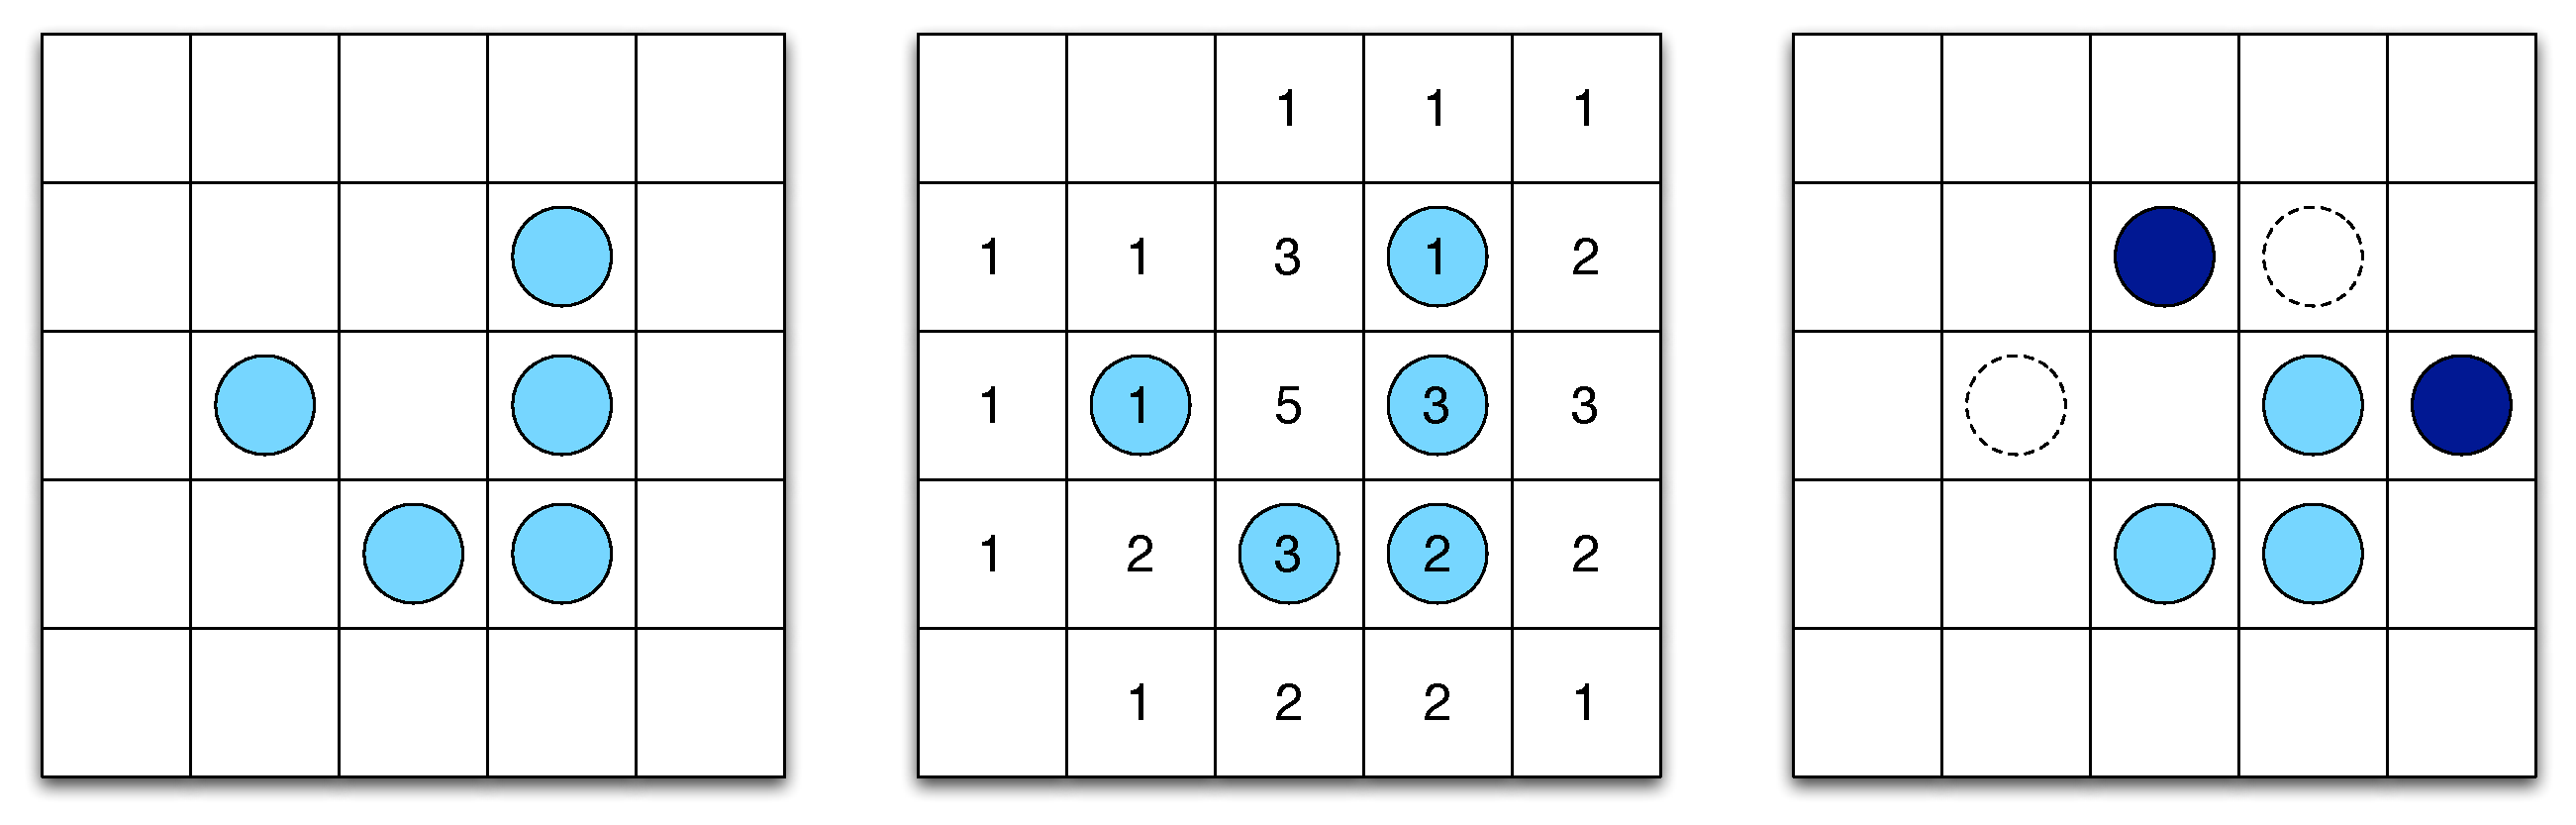
\includegraphics[width=\textwidth]{images/LifeGrid.pdf}

\begin{itemize}
\item Well-known cellular simulation
\item Life and Death based on simple mathematical rules
\item Can we using worker/wrapper and HERMIT to enable agility regarding
our key data-types in the Game of Life?
\end{itemize}
\end{frame}


\begin{frame}[fragile]
\frametitle{HERMIT and the Game of Life}
\Large

HERMIT is a system for applying post-hoc transformations on a Haskell program.
\begin{itemize}
\item Plugin inside GHC
\item REPL shell with a batch mode
\item Lots of commands to transform programs
\item Support for the Worker/wrapper is built-in
\end{itemize}

\frameskip

Can we using worker/wrapper and HERMIT to enable agility regarding
our key data-types in the Game of Life?

\end{frame}


\begin{frame}[fragile]
\frametitle{Hutton's Life}

From Graham Hutton's ``Programming Haskell'':

\begin{codeblock}[0.65]
\tiny
\begin{semiverbatim}
width                         =  20
height                        =  20

type Pos                      = (Int,Int)
type Board                    =  [Pos]

wrap                          :: Pos -> Pos
wrap (x,y)                    =  (((x-1) `mod` width) + 1, ((y-1) `mod` height + 1))

neighbs                       :: Pos -> [Pos]
neighbs (x,y)                 =  map wrap [(x-1,y-1), (x,y-1),
                                           (x+1,y-1), (x-1,y),
                                           (x+1,y)  , (x-1,y+1),
                                           (x,y+1)  , (x+1,y+1)]

isAlive                       :: Board -> Pos -> Bool
isAlive b p                   =  elem p b

isEmpty                       :: Board -> Pos -> Bool
isEmpty b p                   =  not (isAlive b p)

liveneighbs                   :: Board -> Pos -> Int
liveneighbs b                 =  length . filter (isAlive b) . neighbs

survivors                     :: Board -> [Pos]
survivors b                   =  [p | p <- b, elem (liveneighbs b p) [2,3]]

births                        :: Board -> [Pos]
births b                      =  [p | p <- nub (concat (map neighbs b)),
                                      isEmpty b p,
                                      liveneighbs b p == 3]

nextgen                       :: Board -> Board
nextgen b                     =  survivors b ++ births b
\end{semiverbatim}
\end{codeblock}

\end{frame}



\begin{frame}[fragile]
\frametitle{Hutton's Life}
First step, abstract slightly:

\begin{columns}
\begin{column}{0.5\textwidth}

\begin{codeblock}
\tiny
\begin{semiverbatim}
type Pos = (Int,Int)
type Size = (Int,Int)
type Config = (Size,Bool)

class Life b where
        -- create
        empty :: Config -> b
        -- board operations
        diff :: b -> b -> b
        next :: b -> b
        -- point operations
        inv :: Pos -> b -> b
        -- projections
        dims :: b -> Size
        alive :: b -> [Pos]
\end{semiverbatim}
\end{codeblock}


\end{column}
\begin{column}{0.5\textwidth}
\begin{codeblock}
\tiny
\begin{semiverbatim}
type Board = LifeBoard Config [Pos]

...

nextgen :: Board -> Board
nextgen b = LifeBoard (config b) \$ sort
          \$ board (survivors b) ++ board (births b)

instance Life Board where
  empty c = LifeBoard c []
  dims b = fst \$ config b
  diff b1 b2 = LifeBoard (config b1)
             \$ board b1 \\ board b2
  next b = nextgen b
  inv p b = LifeBoard (config b) \$
    if isAlive b p
    then filter ((/=) p) \$ board b
    else sort \$ p : board b
  alive b = board b
\end{semiverbatim}
\end{codeblock}


\end{column}

\end{columns}

\begin{itemize}
\item We tagged Hutton's Board structure with a wrapping boolean.
\item Hutton's Life plugged into the \verb|Life| class, almost verbatim
\item We did sort the list of positions (hope to lift this later)
\end{itemize}

\end{frame}

\begin{frame}[fragile]
\frametitle{Provide {\tt abs} and {\tt rep}}

First example: translating list of (live) positions into a \verb|Set| of life positions.

\begin{codeblock}
\tiny
\begin{semiverbatim}
-- Standard implementation
type Board = LifeBoard Config [Pos]
-- The new data structure to be used in the implementation
type Board' = LifeBoard Config (Set Pos)

-- Transformations required by hermit for worker/wrapper conversions
-- repb and absb change the underlying board field
repb :: [Pos] -> Set Pos
repb = fromDistinctAscList

absb :: Set Pos -> [Pos]
absb = toAscList

-- repB and absB change the entire Board structure
repB :: Board -> Board'
repB b = LifeBoard (config b) \$ repb (board b)

absB :: Board' -> Board
absB b = LifeBoard (config b) \$ absb (board b)

-- representation of (Board -> Board) "births", "survivors", "nextgen", "next"
repBB :: (Board -> Board) -> (Board' -> Board')
repBB = repBx . repxB

-- abstraction of (Board' -> Board') "births", "survivors", "nextgen", "next"
absBB :: (Board' -> Board') -> (Board -> Board)
absBB = absBx . absxB

...
\end{semiverbatim}
\end{codeblock}

\end{frame}

\begin{frame}[fragile]
\frametitle{Apply worker/wrapper using HERMIT}

(Warning: Real Code)

\begin{codeblock}
\tiny
\begin{verbatim}
binding-of 'nextgen
fix-intro
down
split-1-beta nextgen [|absBB|] [|repBB|]
{
  rhs-of 'g
  repeat (any-call (unfold ['births, 'survivors, 'absBB, 'repBB]))
  bash
  one-td let-subst
  any-call (unfold-rule config-absB)
  any-call (unfold-rule board-absB)
  any-call (unfold-rule sort-++-absb)
  any-call (unfold-rule LifeBoard-absb)
  any-call (unfold-rule repB-absB)
}
let-subst
alpha-let ['nextgen']
{ let-bind ; nonrec-rhs ; unfold ; bash }
top
innermost let-float
\end{verbatim}
\end{codeblock}

\frameskip

Example GHC RULE:

{\tiny
\begin{verbatim}
          {-# RULES "sort-++-absb" [~] forall b1 b2. sort (absb b1 ++ absb b2) = absb (union b1 b2) #-}
\end{verbatim}
}


\end{frame}


\begin{frame}[fragile]
\frametitle{Other Datatypes}

We have converted the Game of Life to 3 different representations.

\frameskip

\begin{itemize}
\item \verb|Set (Int,Int)| -- Haskell's \verb|Set| representation.
\item QuadTree Bool -- 2D binary hierarchical space subdivision of a region.
\item UVector Bool -- a packed unboxed vector of bits.
\end{itemize}

\frameskip

Can we translate to more novel structures?

\end{frame}

\begin{frame}[fragile]
\frametitle{Accelerate!}

Accelerate is a library for translating a subset of Haskell for GPGPUs.

\begin{itemize}
\item Critical type is \verb|Acc|, which represents a computation on the CPU.
\end{itemize}

\begin{codeblock}[0.8]
\begin{verbatim}
data Board = LifeBoard Config [Pos]

data Board' = LifeBoard Config (Acc (Array DIM2 Int))
\end{verbatim}
\end{codeblock}


\frameskip
\begin{itemize}
\item Ongoing work.

\item with this transformation, we can write in non-idiomatic Haskell,
and manage to run the result on a GPU.
\end{itemize}


\begin{codeblock}[1]
\begin{verbatim}
run :: Arrays a => Acc a -> a
run1 :: (Arrays a, Arrays b) => (Acc a -> Acc b) -> a -> b
stream :: (Arrays a, Arrays b) => (Acc a -> Acc b) -> [a] -> [b]
\end{verbatim}
\end{codeblock}


\end{frame}


\begin{frame}
\frametitle{Conclusions}

\begin{itemize}
\item Worker/wrapper is a general and systematic approach to transforming
a computation of one type into an equivalent computation of another type.

\item We have used worker/wrapper and HERMIT to translate
between different representations of a Game of Life board.

\item The process was tedious, but the same pattern was used again and again.

\item Next steps:
\begin{itemize}
\item More powerful abstractions for worker/wrapper and abs/rep generation.
\item Mapping to the GPU.
\end{itemize}

\end{itemize}

\end{frame}

%\begin{frame}
%\frametitle{Further Work}
%
%\begin{itemize}
%\item Monadic and Effectful Constructions
%\item Mechanization
%\item Implement inside the Haskell Equational Reasoning Assistant
%\item Consider other patterns of recursion
%\end{itemize}
%
%\end{frame}

\end{document}
